\section{Results}
\label{sec:results}

To visualize persistences of homology groups we used the bar code diagrams and
persistence diagrams. The bar code diagram for a certain homology group $H$ is
a two dimensional plot that shows us the life spans of all the homology
classes. For each homology class $\gamma$ we plot a line segment that starts in
point $(i_{\gamma}, y_{\gamma})$ and ends in point $(j_{\gamma}, y_{\gamma})$,
where $i_{\gamma}$ and $j_{\gamma}$ are life and death of $\gamma$ and
$y_{\gamma}$ is a unique number that represents $\gamma$ on the $y$ axis of the
plot.

Persistence diagrams show the same information in the form of a scatter plot.
For each $\gamma$, $pers(\gamma) = [i_{\gamma}, j_{\gamma}]$ in some homology
group we just plot the point $(i_{\gamma}, j_{\gamma})$.

Here are the barcode diagrams and persistence diagrams obtained for each of the
three domains abstracts, sports and reviews. To generate this specific plots we
used all the feature functions described in~\ref{sub:preparation_of_data} plus
the tf-idf method for the first $50$ most common words. We also used the
maximal filtration, meaning filtration (in particular parameter $r$) was not
split to some predetermined number of intervals but just left as is and in this
case we were looking at the formations of Čech complexes.

%***********%
% abstracts %
%***********%

\begin{figure}[H]
  \centering
  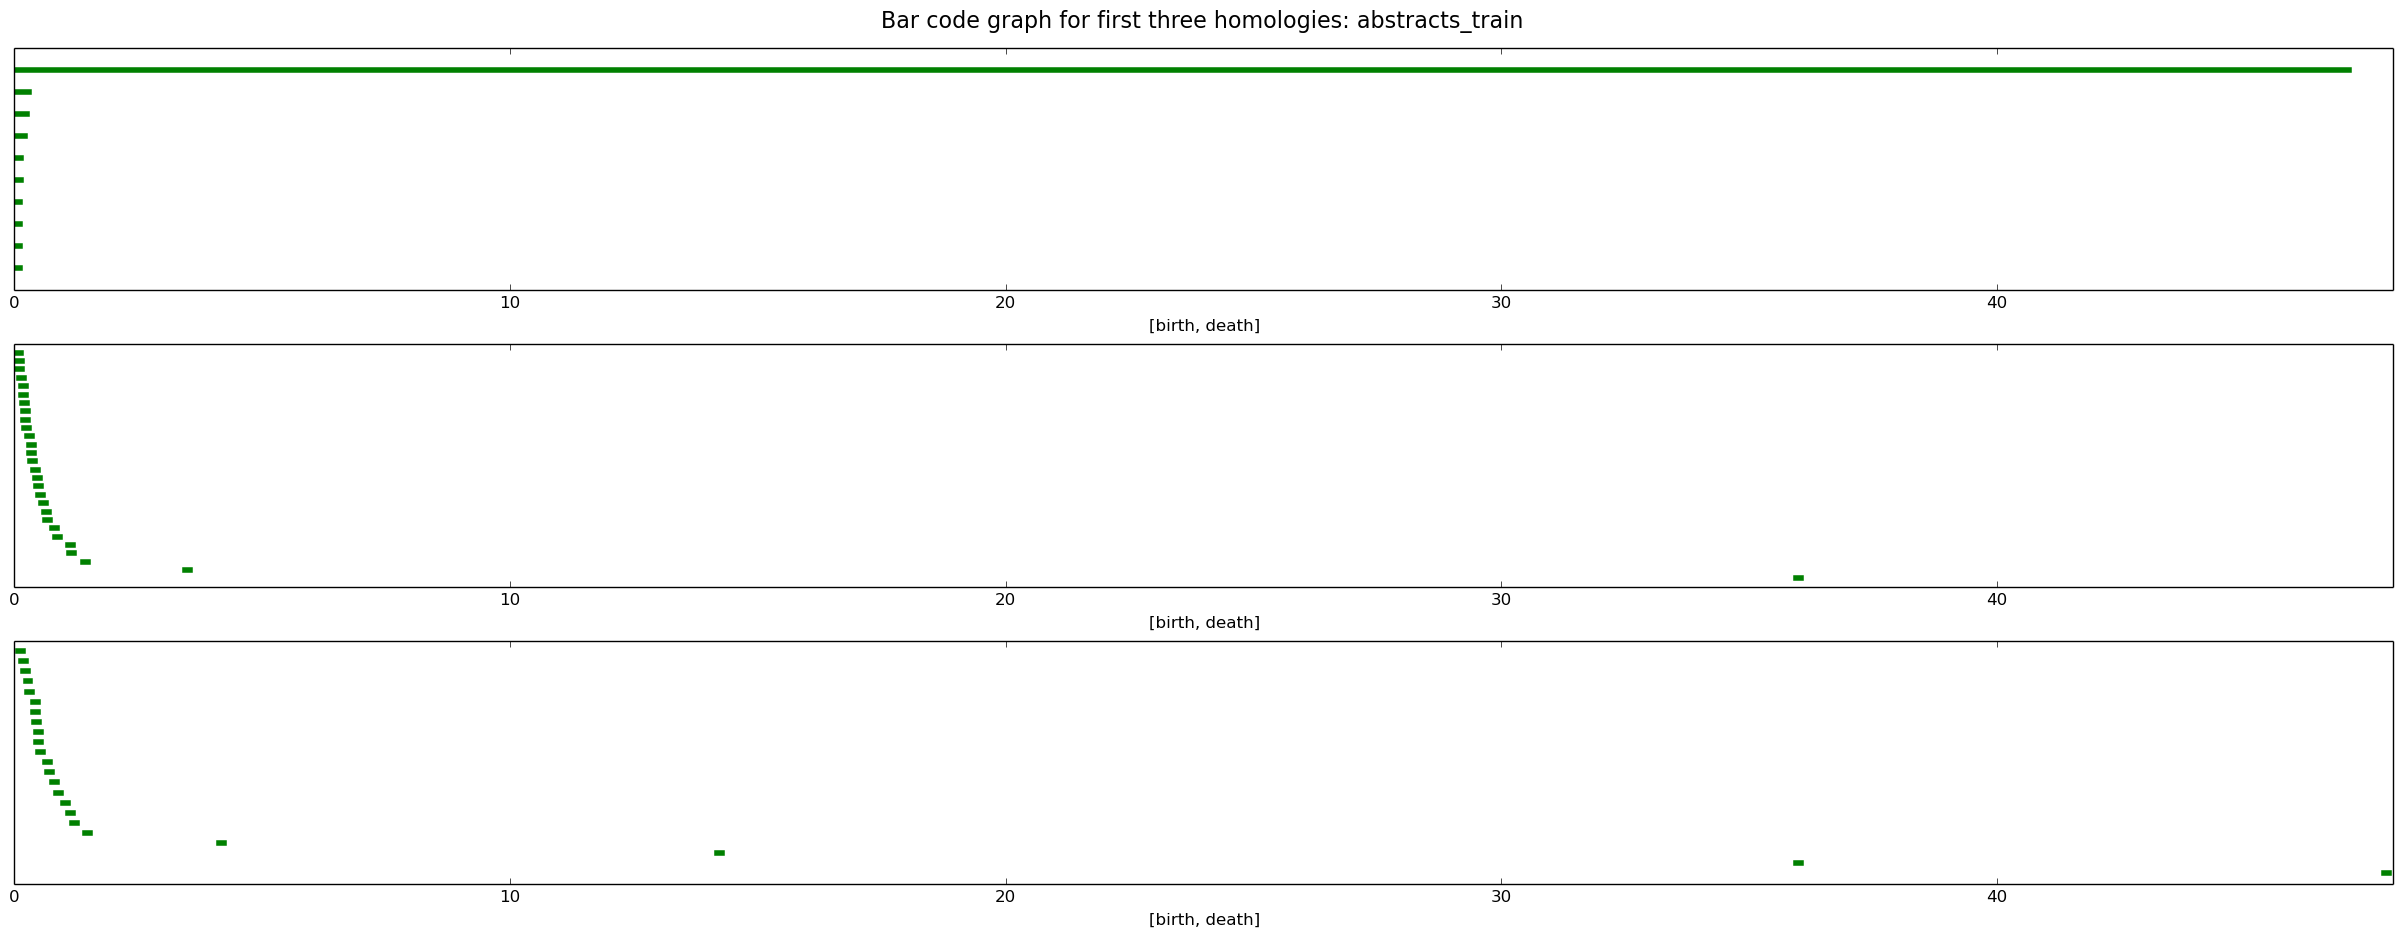
\includegraphics[width=\textwidth]{{img/bar_code_diagram_abstracts_train.png}}
  \caption{Bar codes for abstracts\_train}
  \label{fig:a_1}
\end{figure}

\begin{figure}[H]
  \centering
  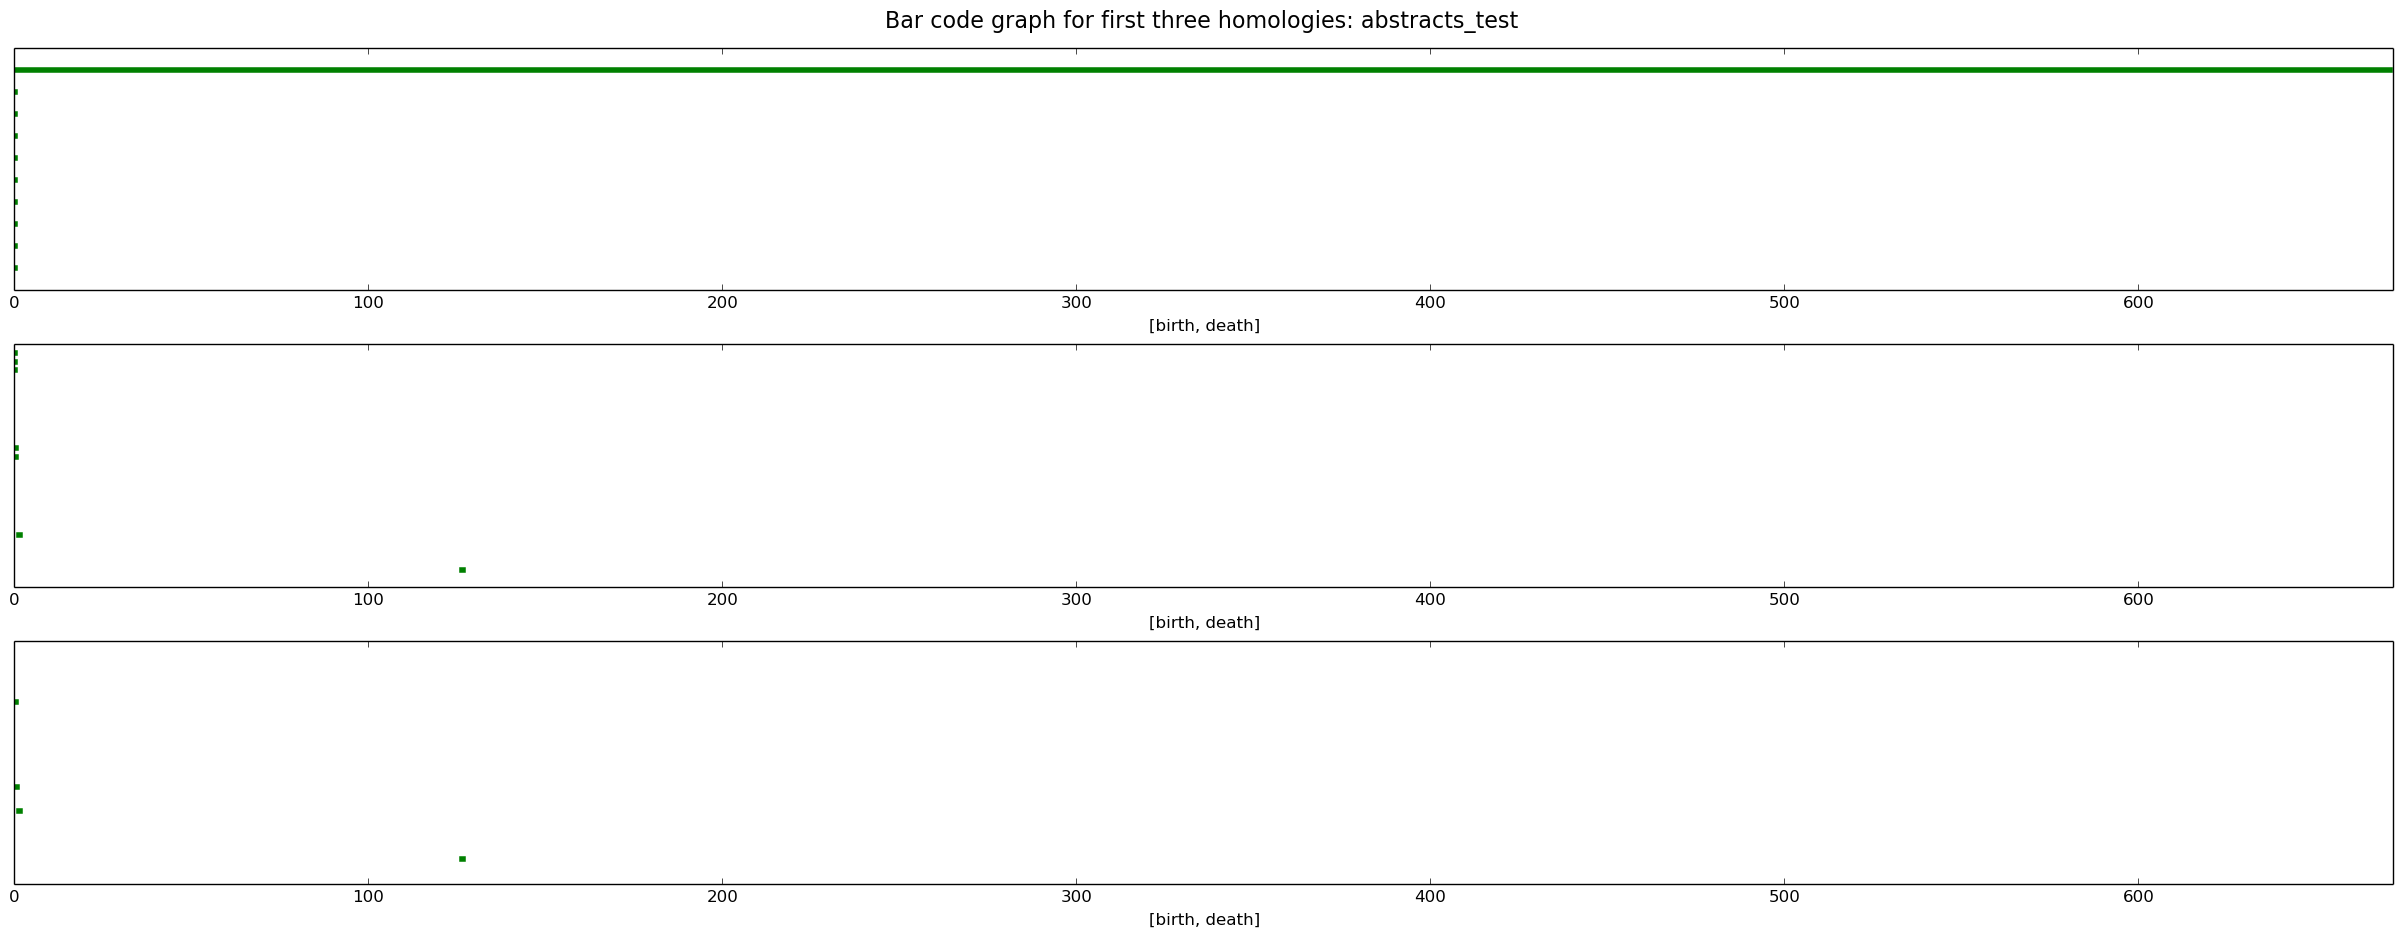
\includegraphics[width=\textwidth]{{img/bar_code_diagram_abstracts_test.png}}
  \caption{Bar codes for abstracts\_test}
  \label{fig:a_2}
\end{figure}

\begin{figure}[H]
  \centering
  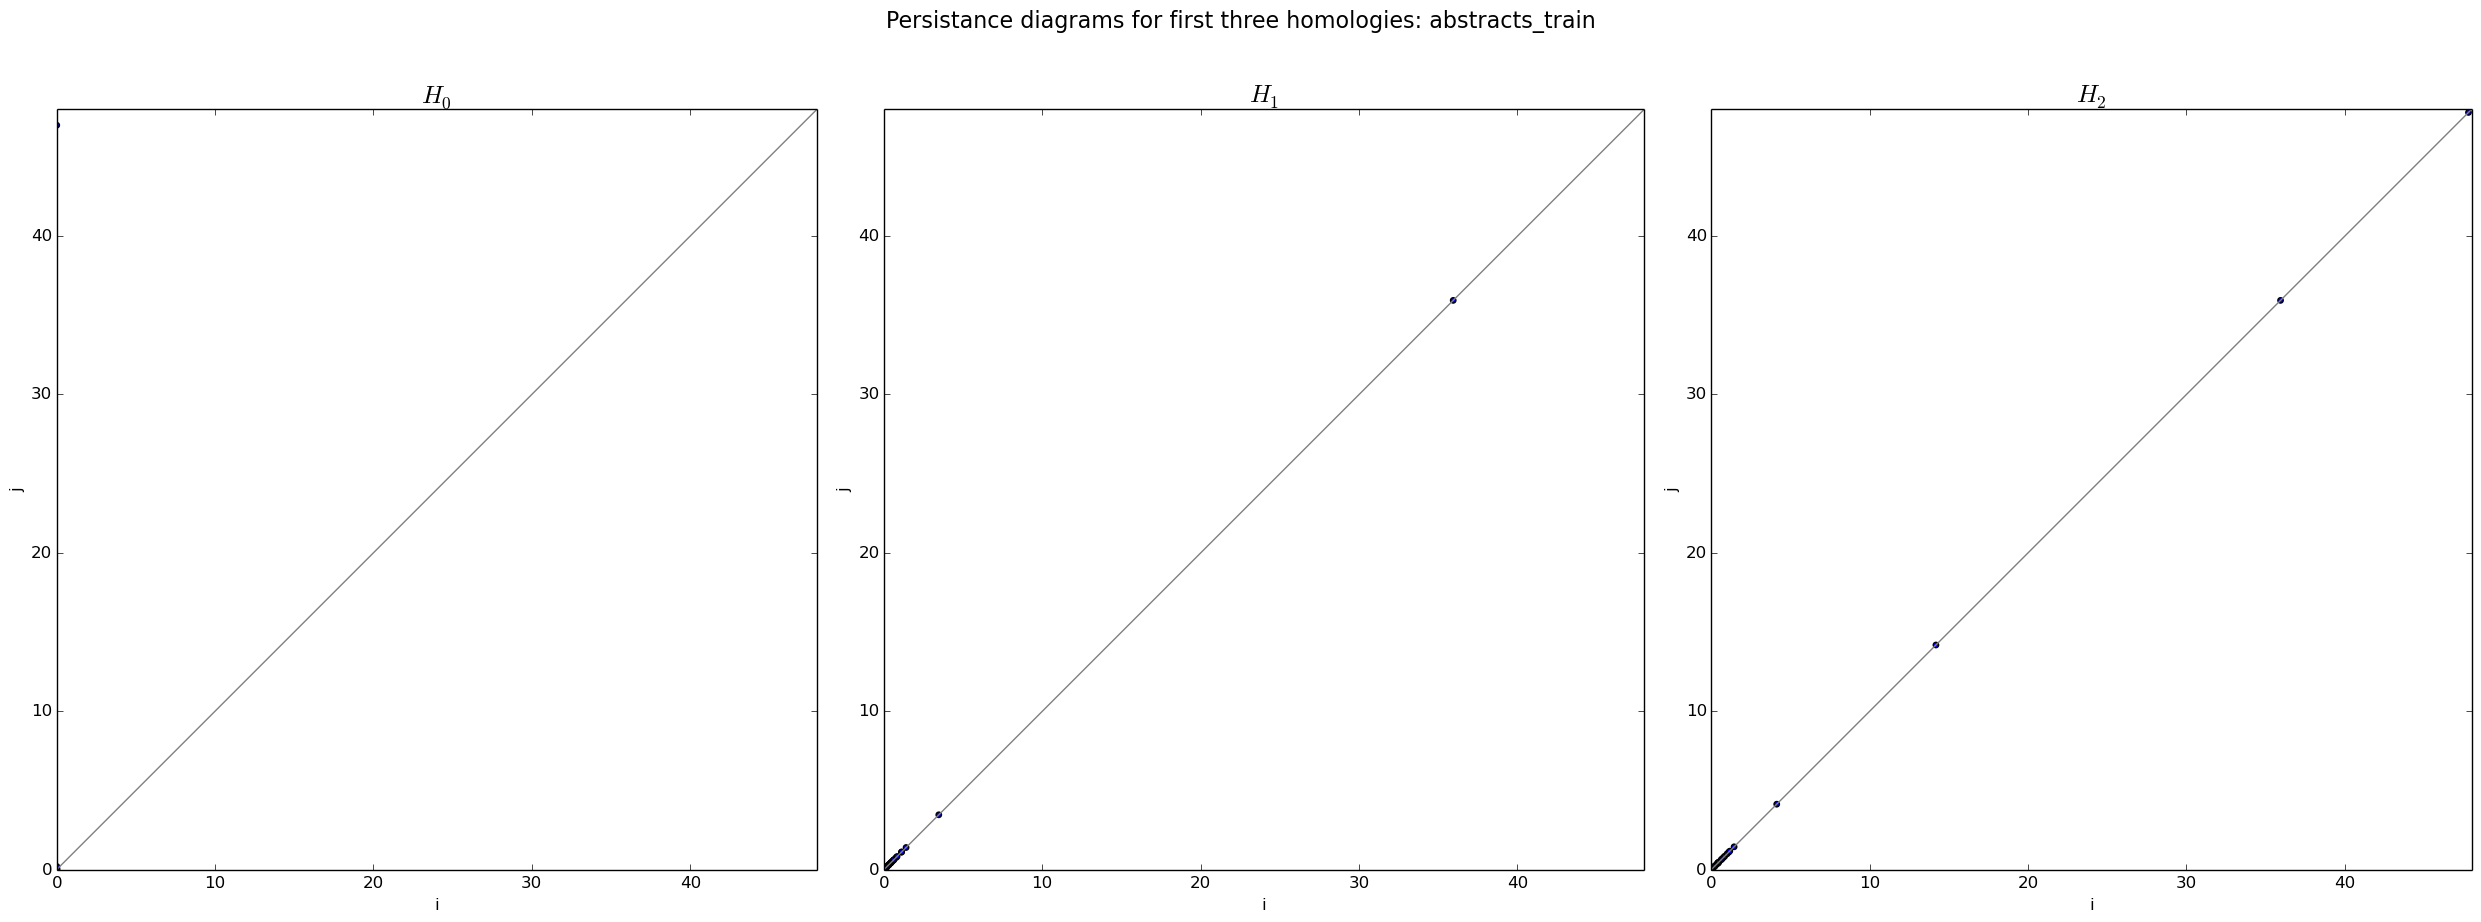
\includegraphics[width=\textwidth]{{img/pers_diagram_abstracts_train.png}}
  \caption{Persistence diagrams for abstracts\_train}
  \label{fig:a_3}
\end{figure}

\begin{figure}[H]
  \centering
  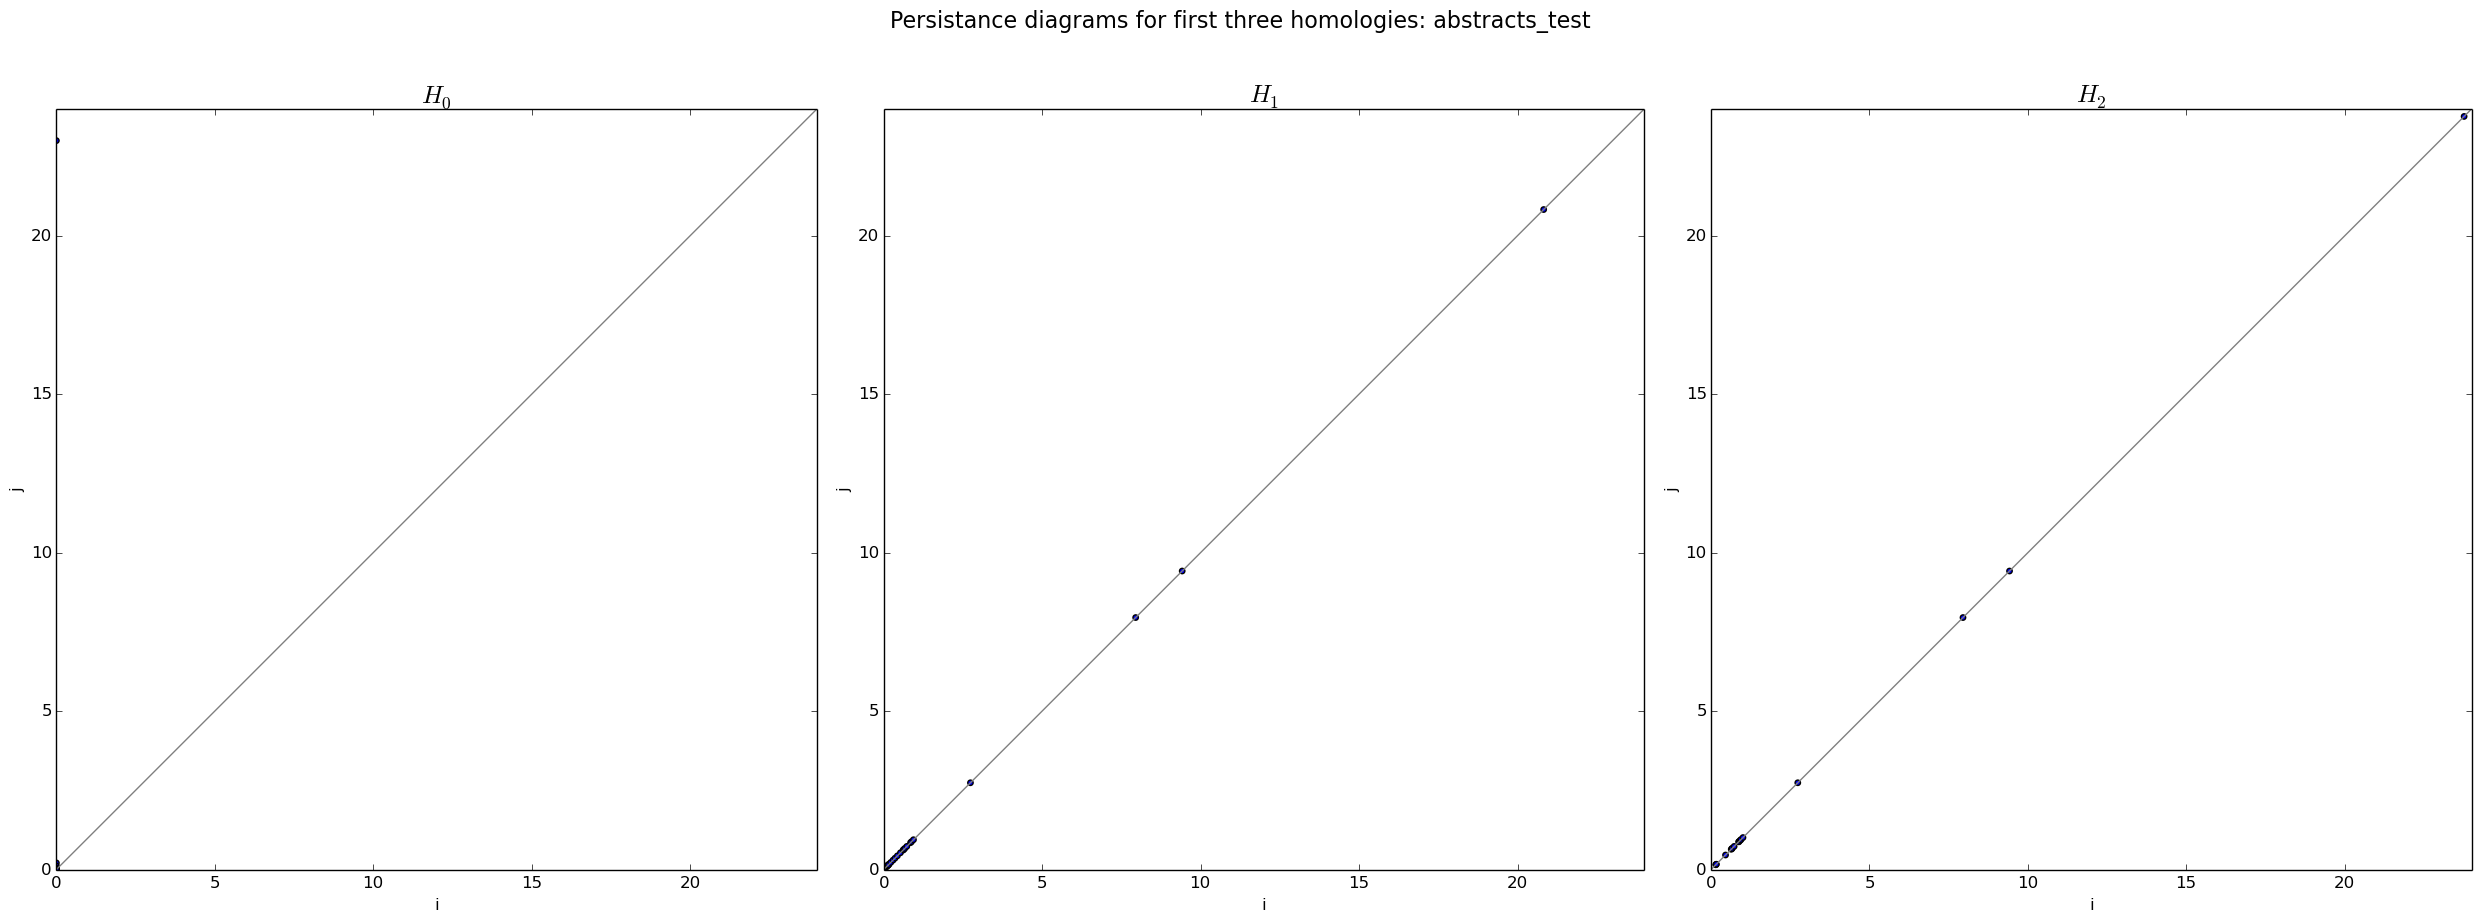
\includegraphics[width=\textwidth]{{img/pers_diagram_abstracts_test.png}}
  \caption{Persistence diagrams for abstracts\_test}
  \label{fig:a_4}
\end{figure}

%********%
% sports %
%********%

\begin{figure}[H]
  \centering
  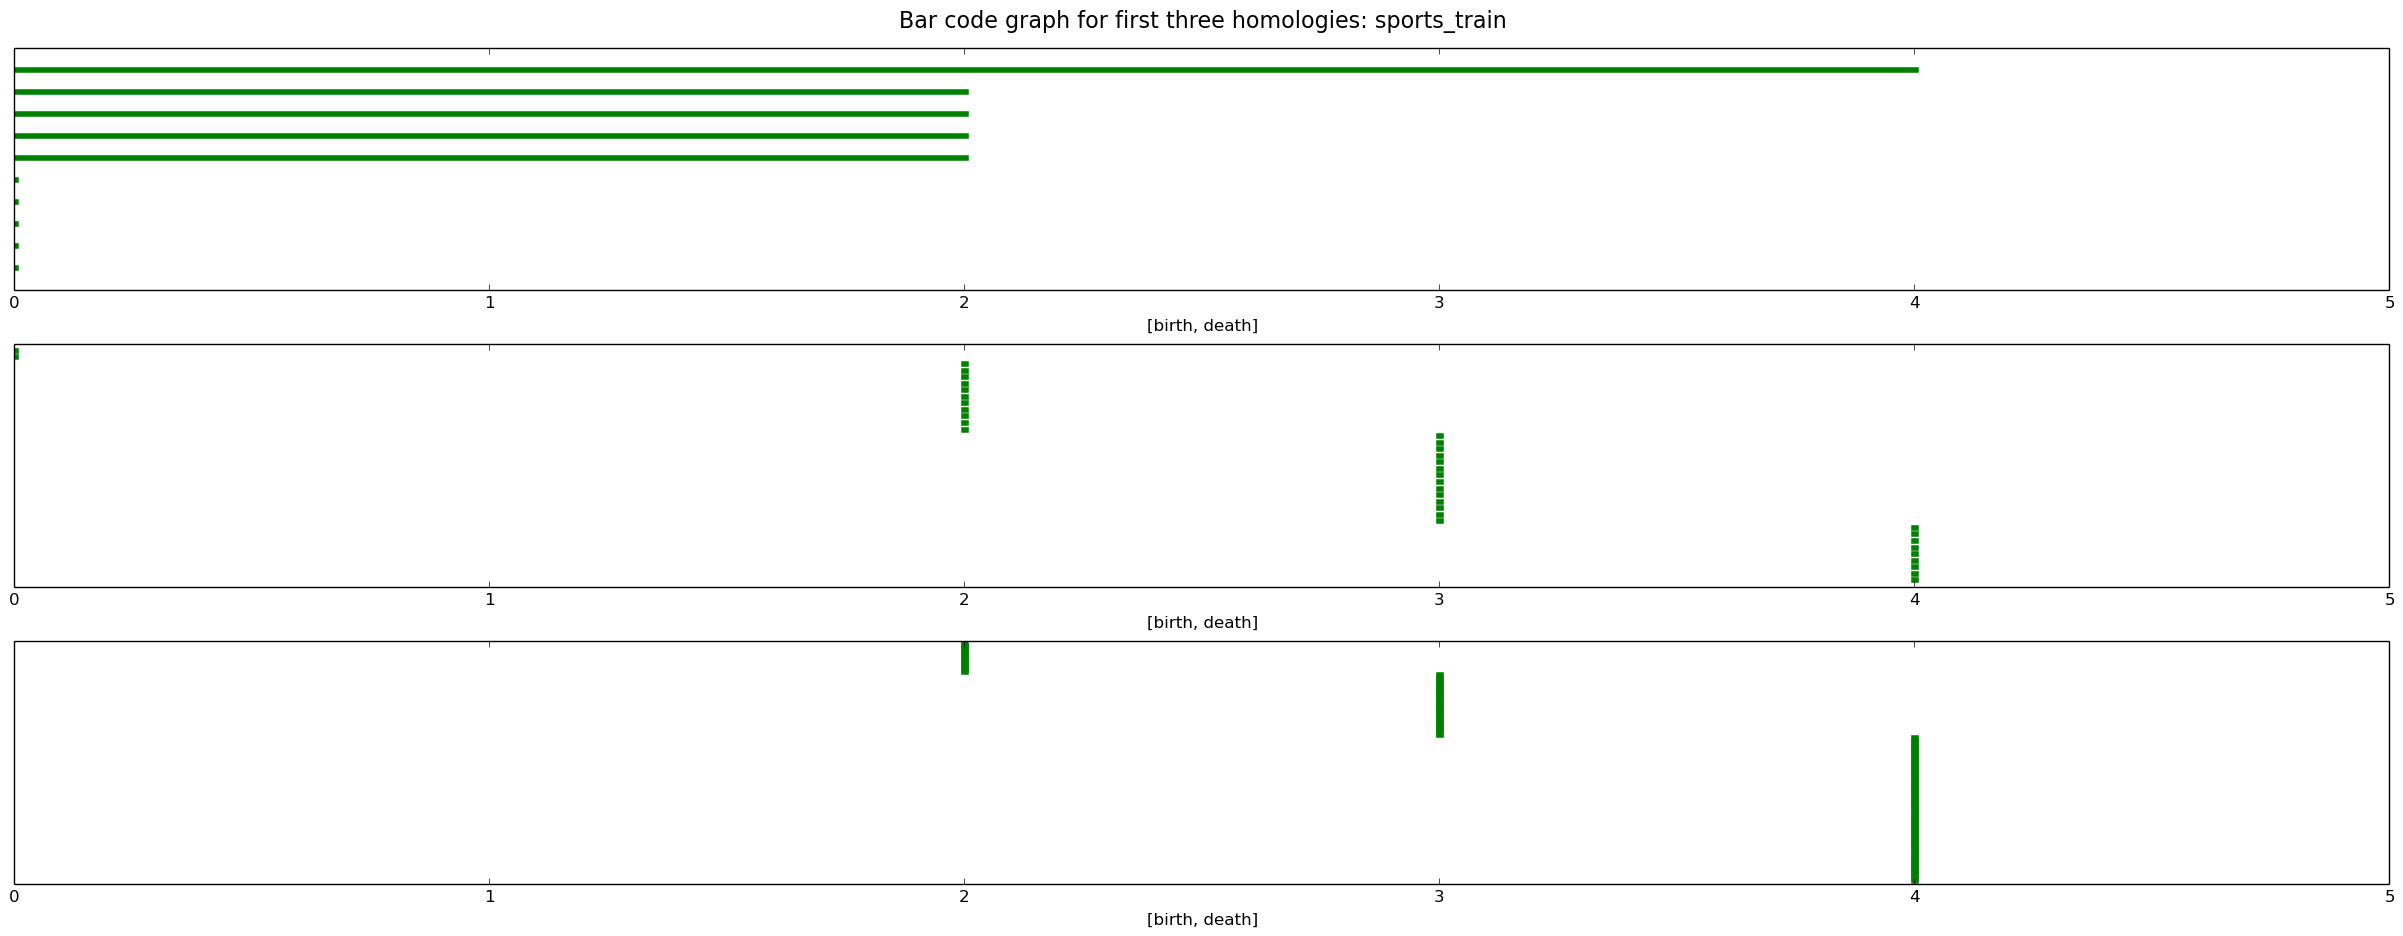
\includegraphics[width=\textwidth]{{img/bar_code_diagram_sports_train.png}}
  \caption{Bar codes for sports\_train}
  \label{fig:s_1}
\end{figure}

\begin{figure}[H]
  \centering
  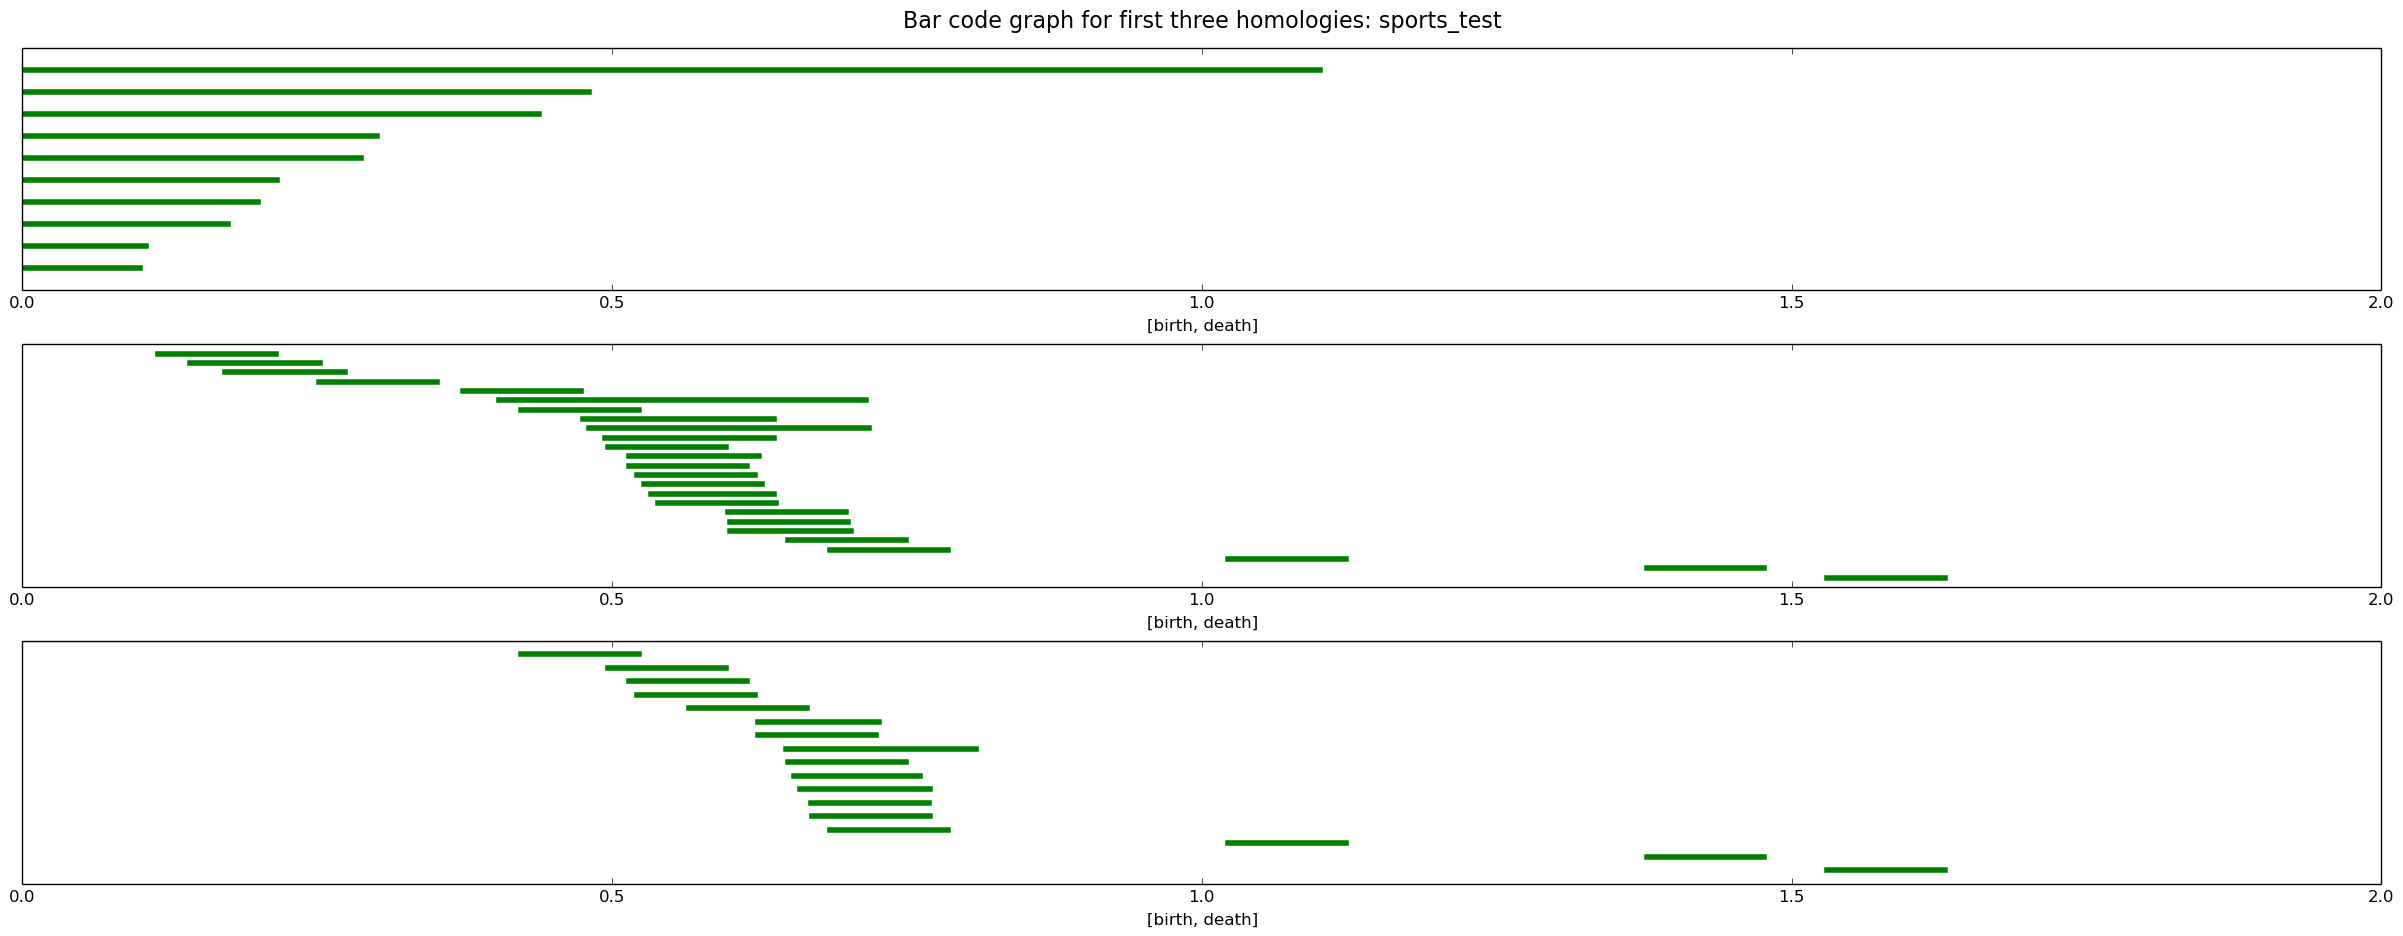
\includegraphics[width=\textwidth]{{img/bar_code_diagram_sports_test.png}}
  \caption{Bar codes for sports\_test}
  \label{fig:s_2}
\end{figure}

\begin{figure}[H]
  \centering
  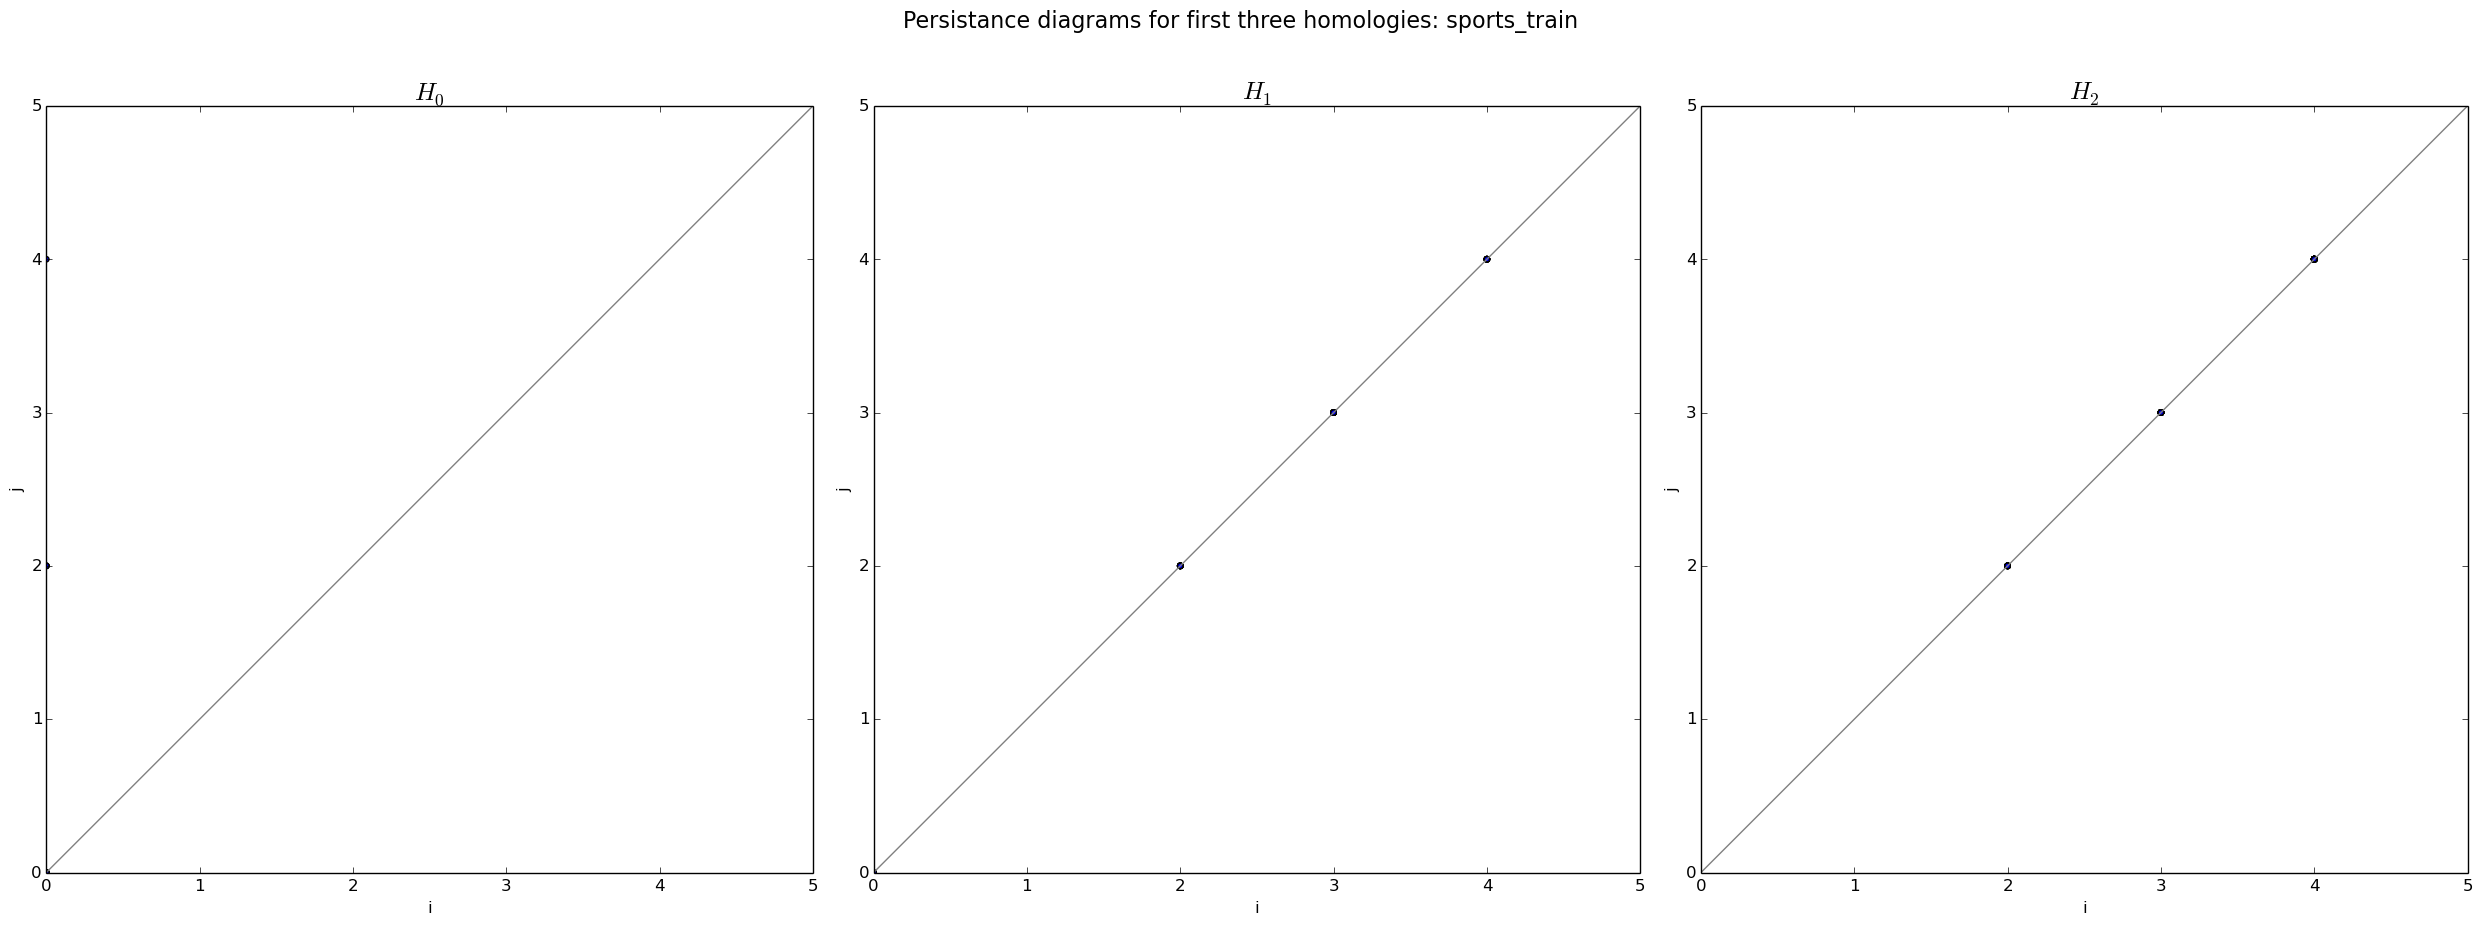
\includegraphics[width=\textwidth]{{img/pers_diagram_sports_train.png}}
  \caption{Persistence diagrams for sports\_train}
  \label{fig:s_3}
\end{figure}

\begin{figure}[H]
  \centering
  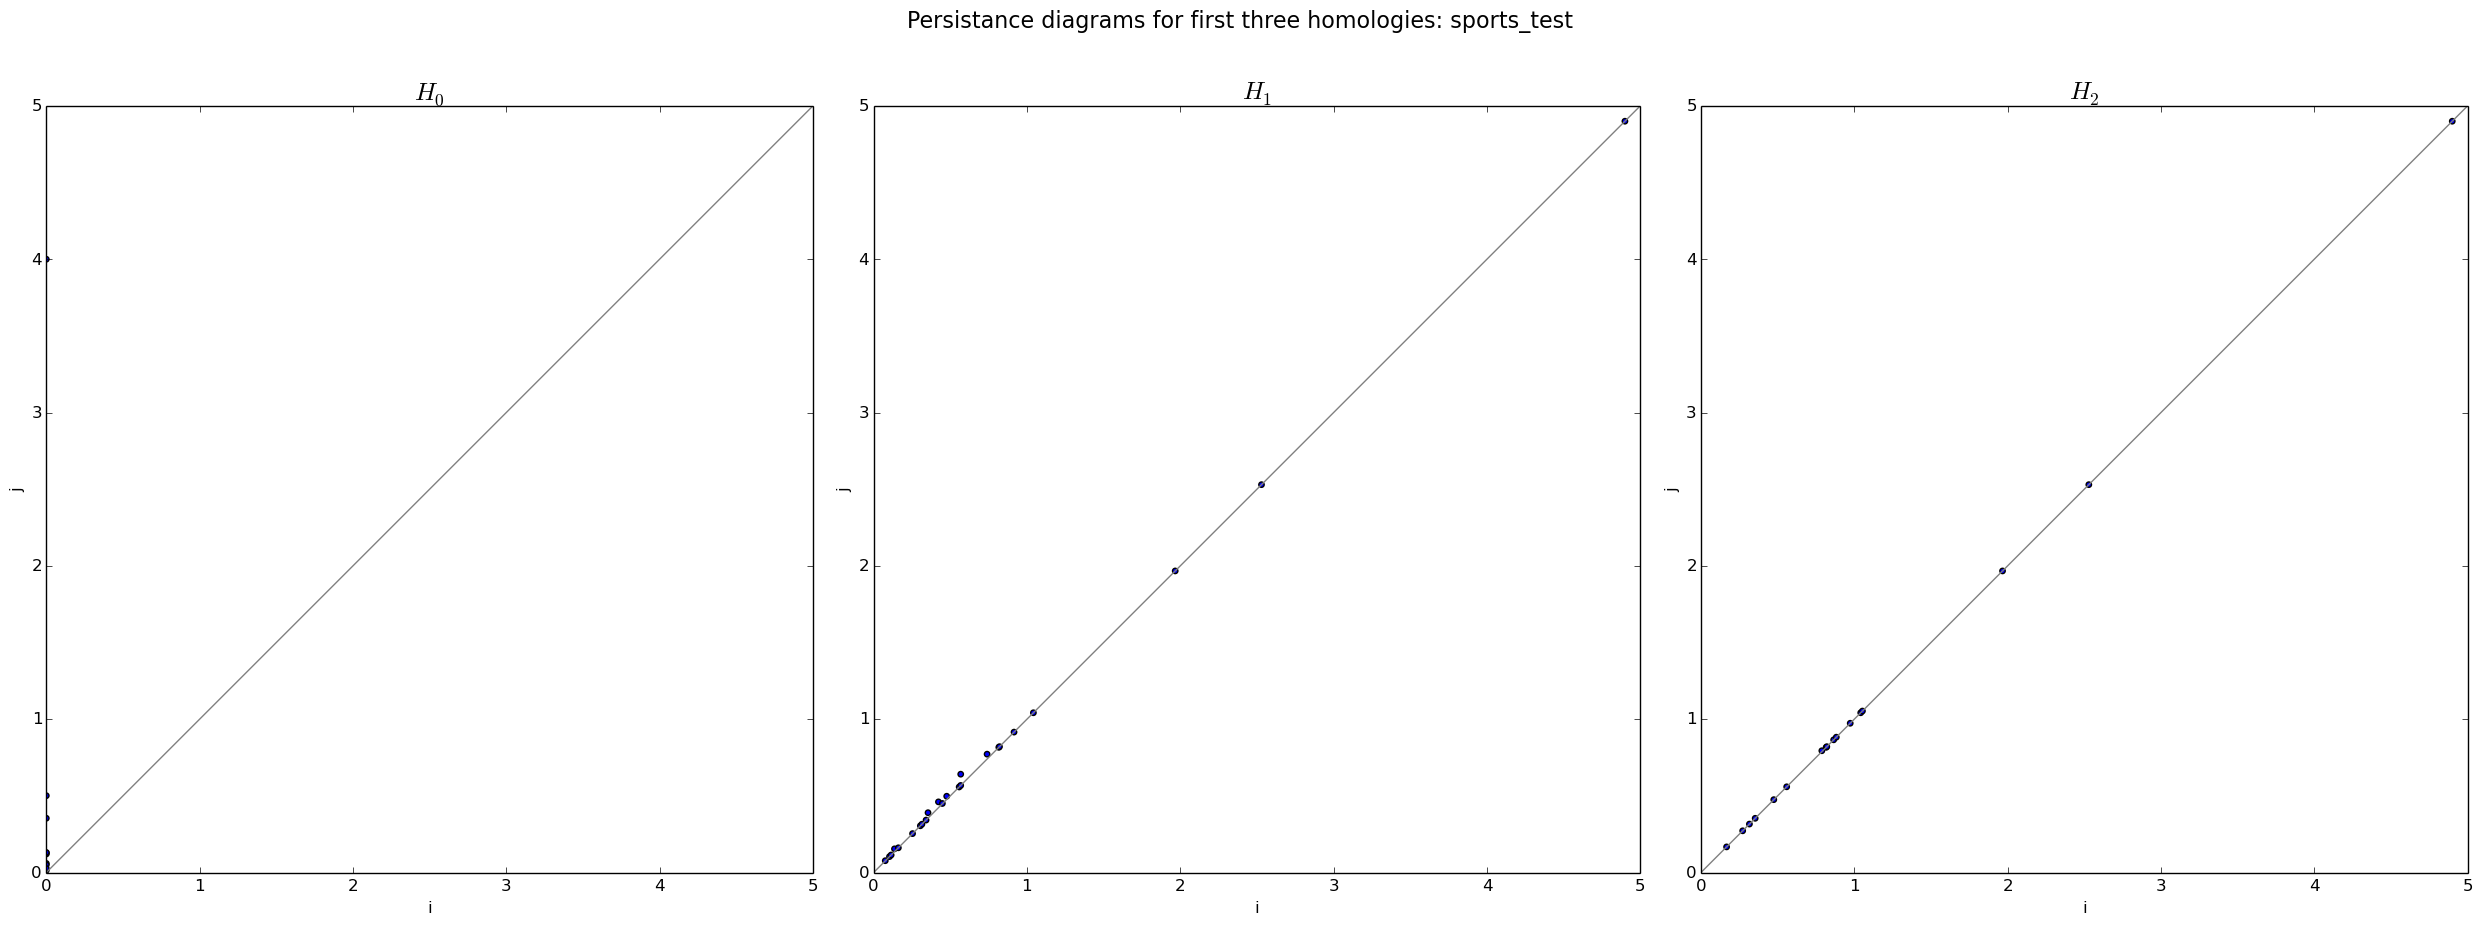
\includegraphics[width=\textwidth]{{img/pers_diagram_sports_test.png}}
  \caption{Persistence diagrams for sports\_test}
  \label{fig:s_4}
\end{figure}

%*********%
% reviews %
%*********%

\begin{figure}[H]
  \centering
  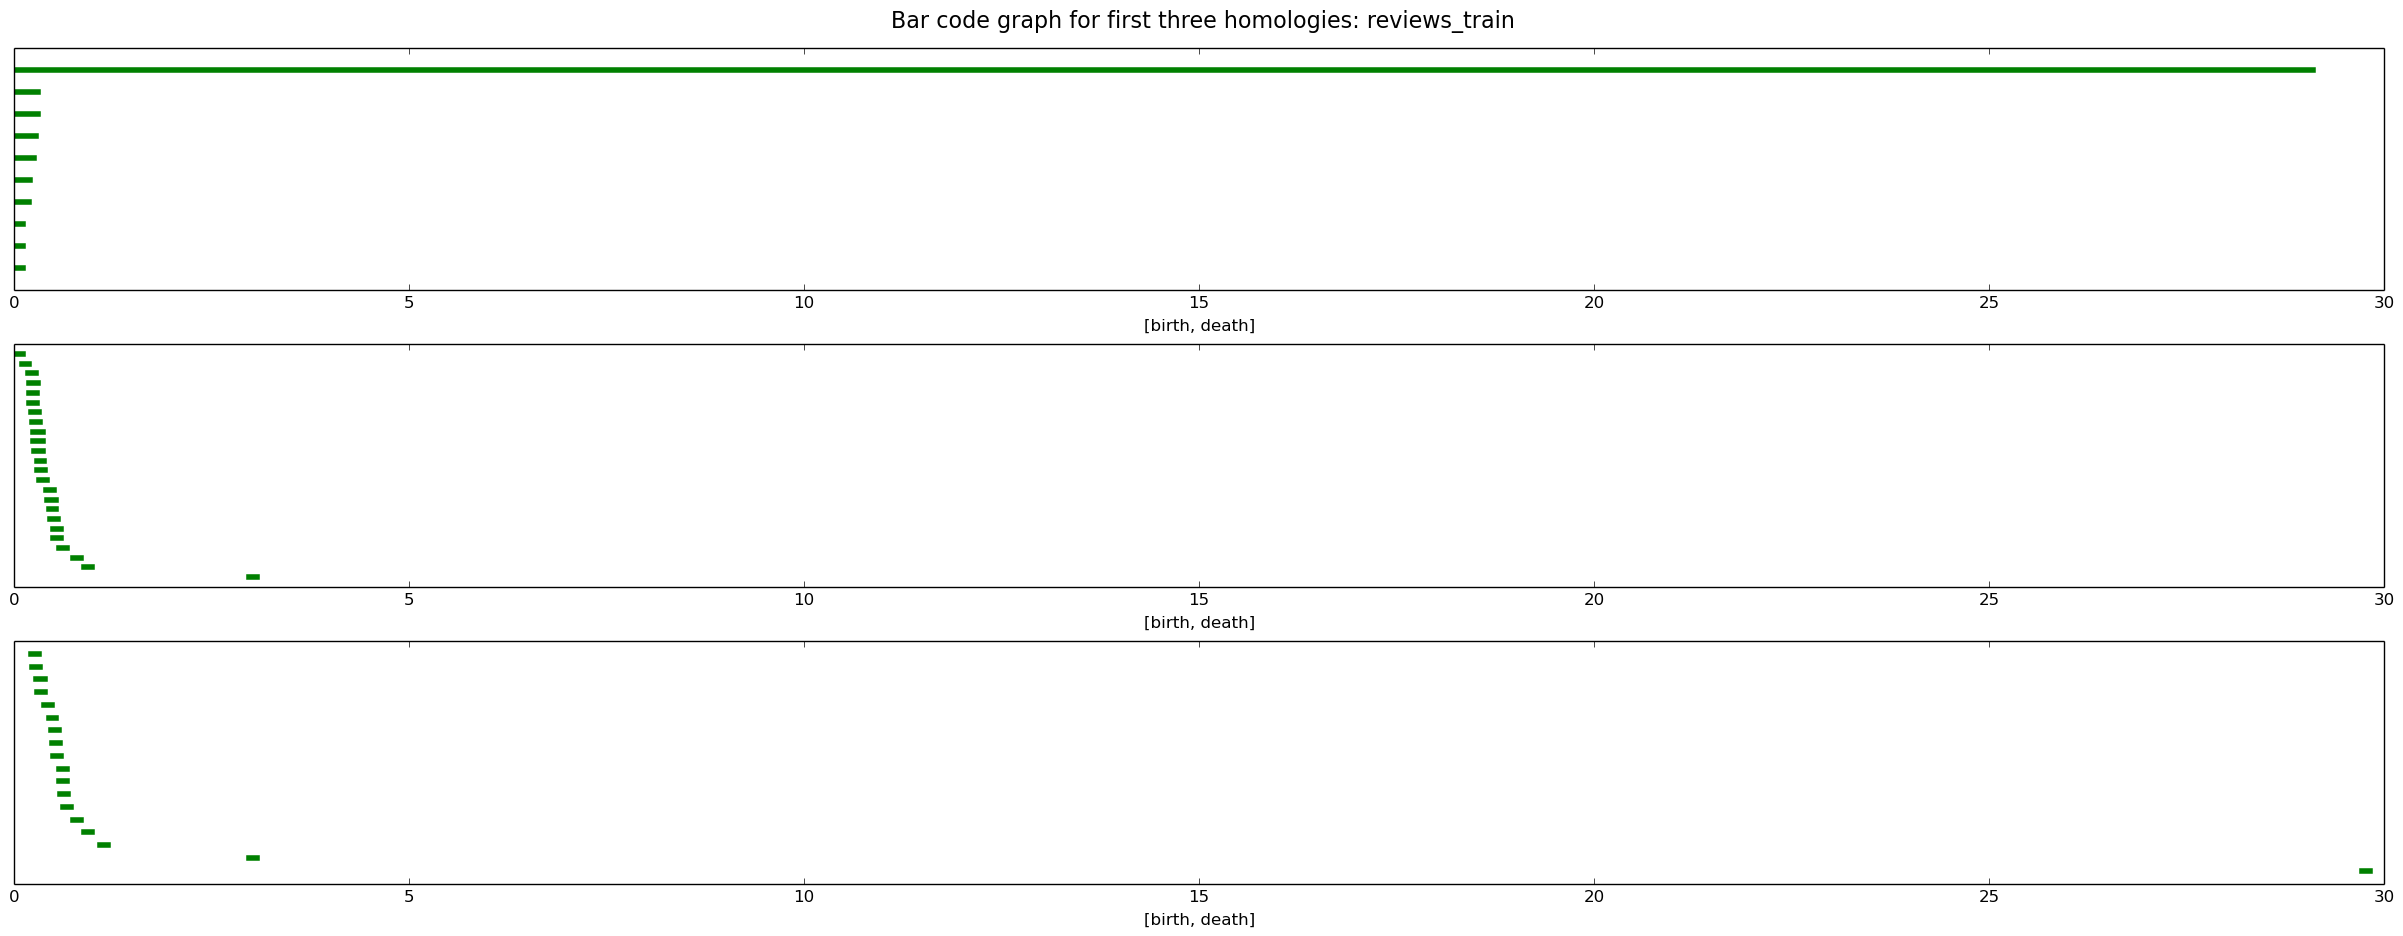
\includegraphics[width=\textwidth]{{img/bar_code_diagram_reviews_train.png}}
  \caption{Bar codes for reviews\_train}
  \label{fig:s_1}
\end{figure}

\begin{figure}[H]
  \centering
  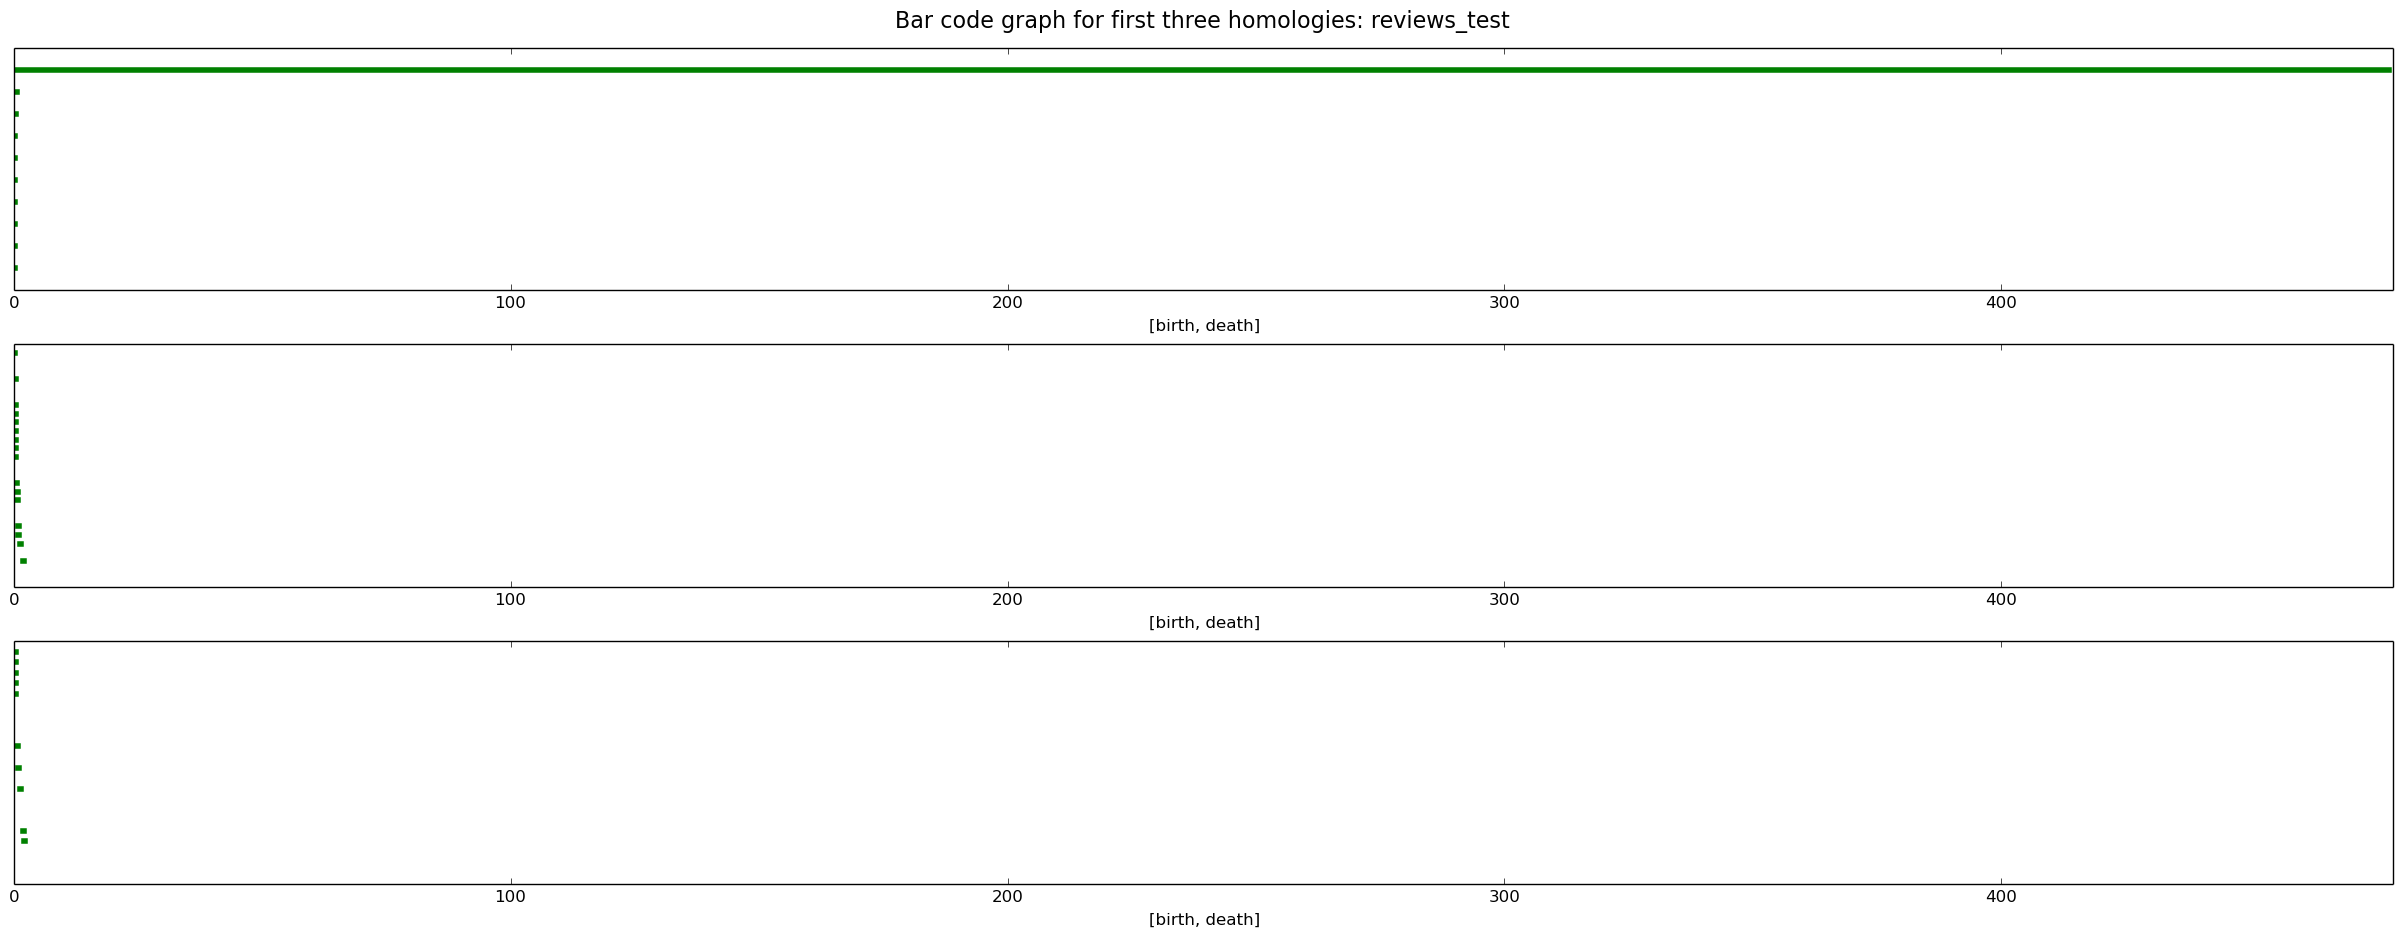
\includegraphics[width=\textwidth]{{img/bar_code_diagram_reviews_test.png}}
  \caption{Bar codes for reviews\_test}
  \label{fig:s_2}
\end{figure}

\begin{figure}[H]
  \centering
  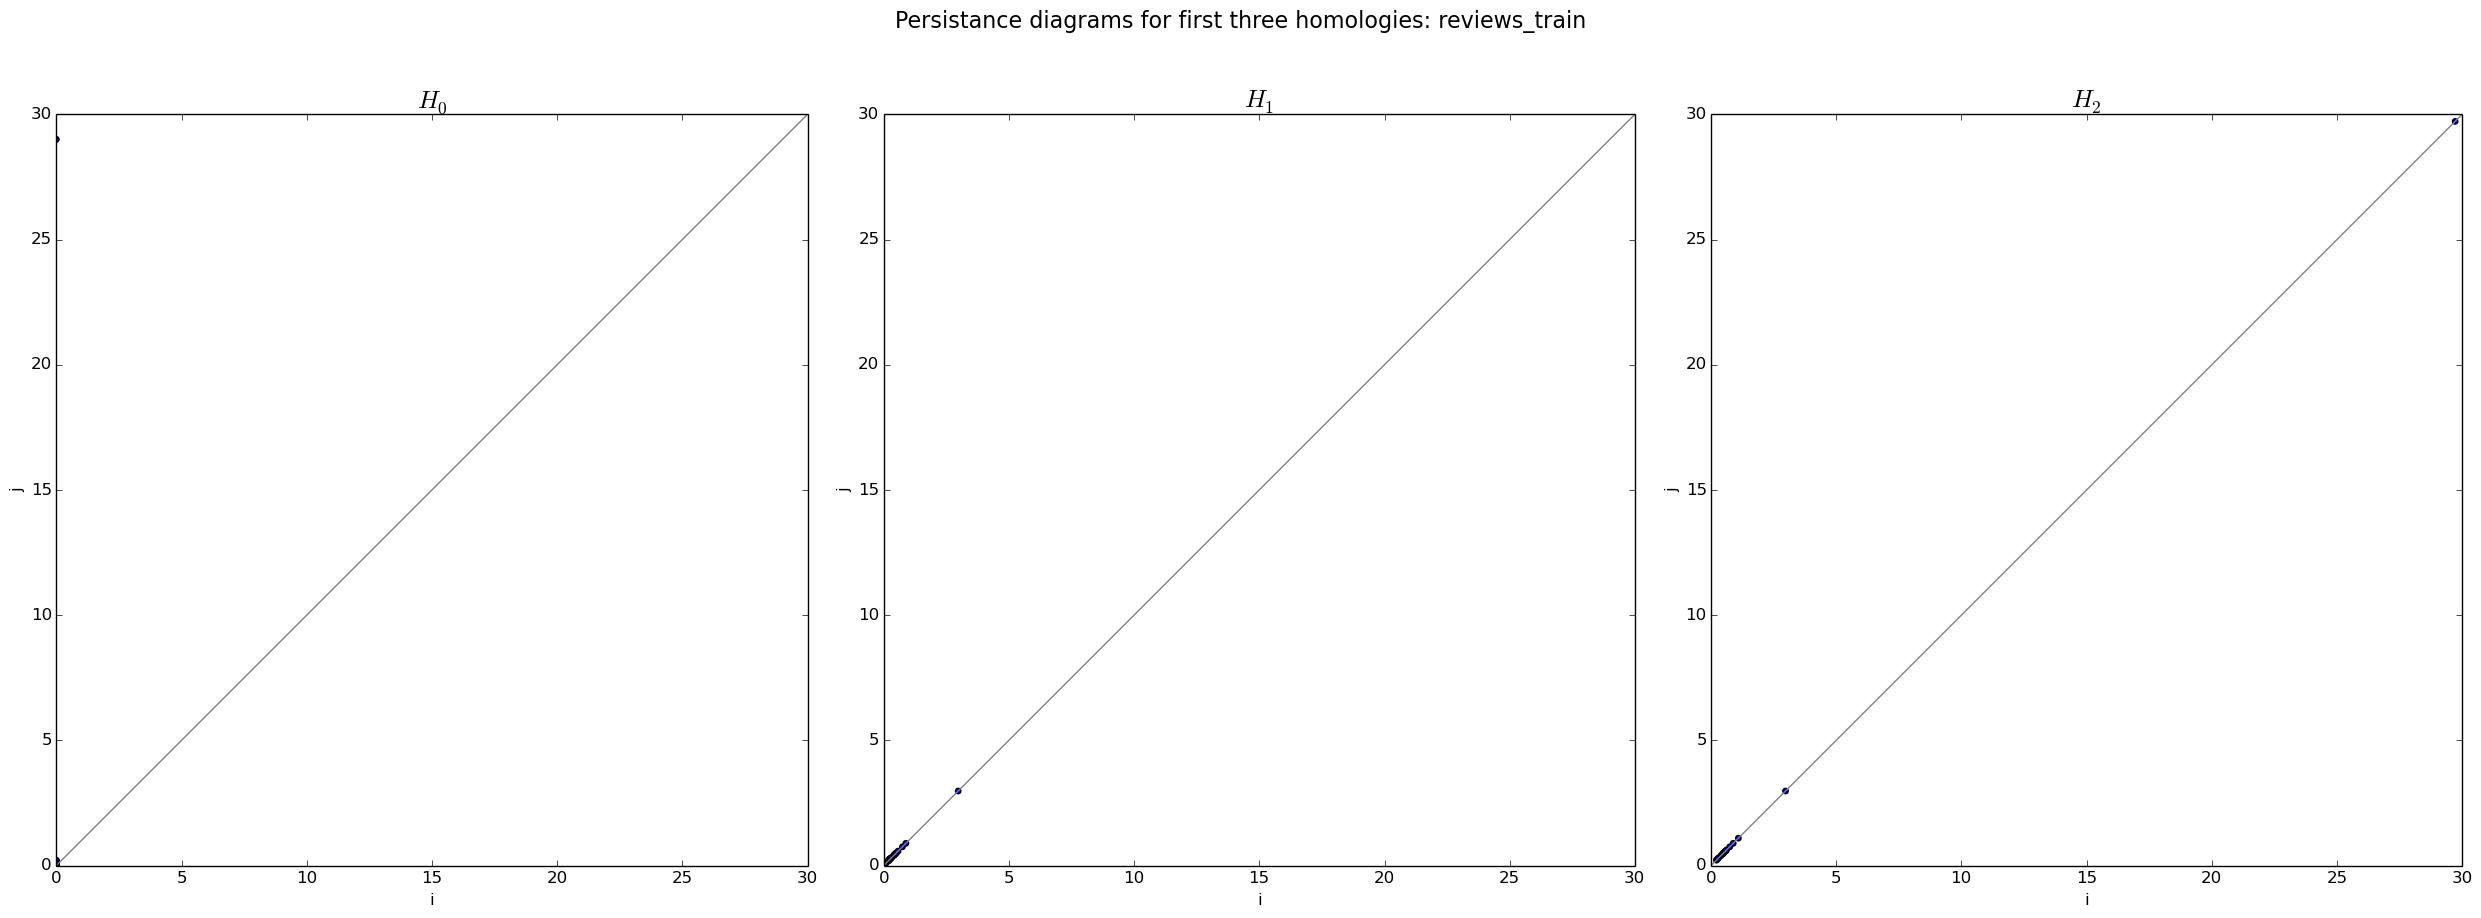
\includegraphics[width=\textwidth]{{img/pers_diagram_reviews_train.png}}
  \caption{Persistence diagrams for reviews\_train}
  \label{fig:s_3}
\end{figure}

\begin{figure}[H]
  \centering
  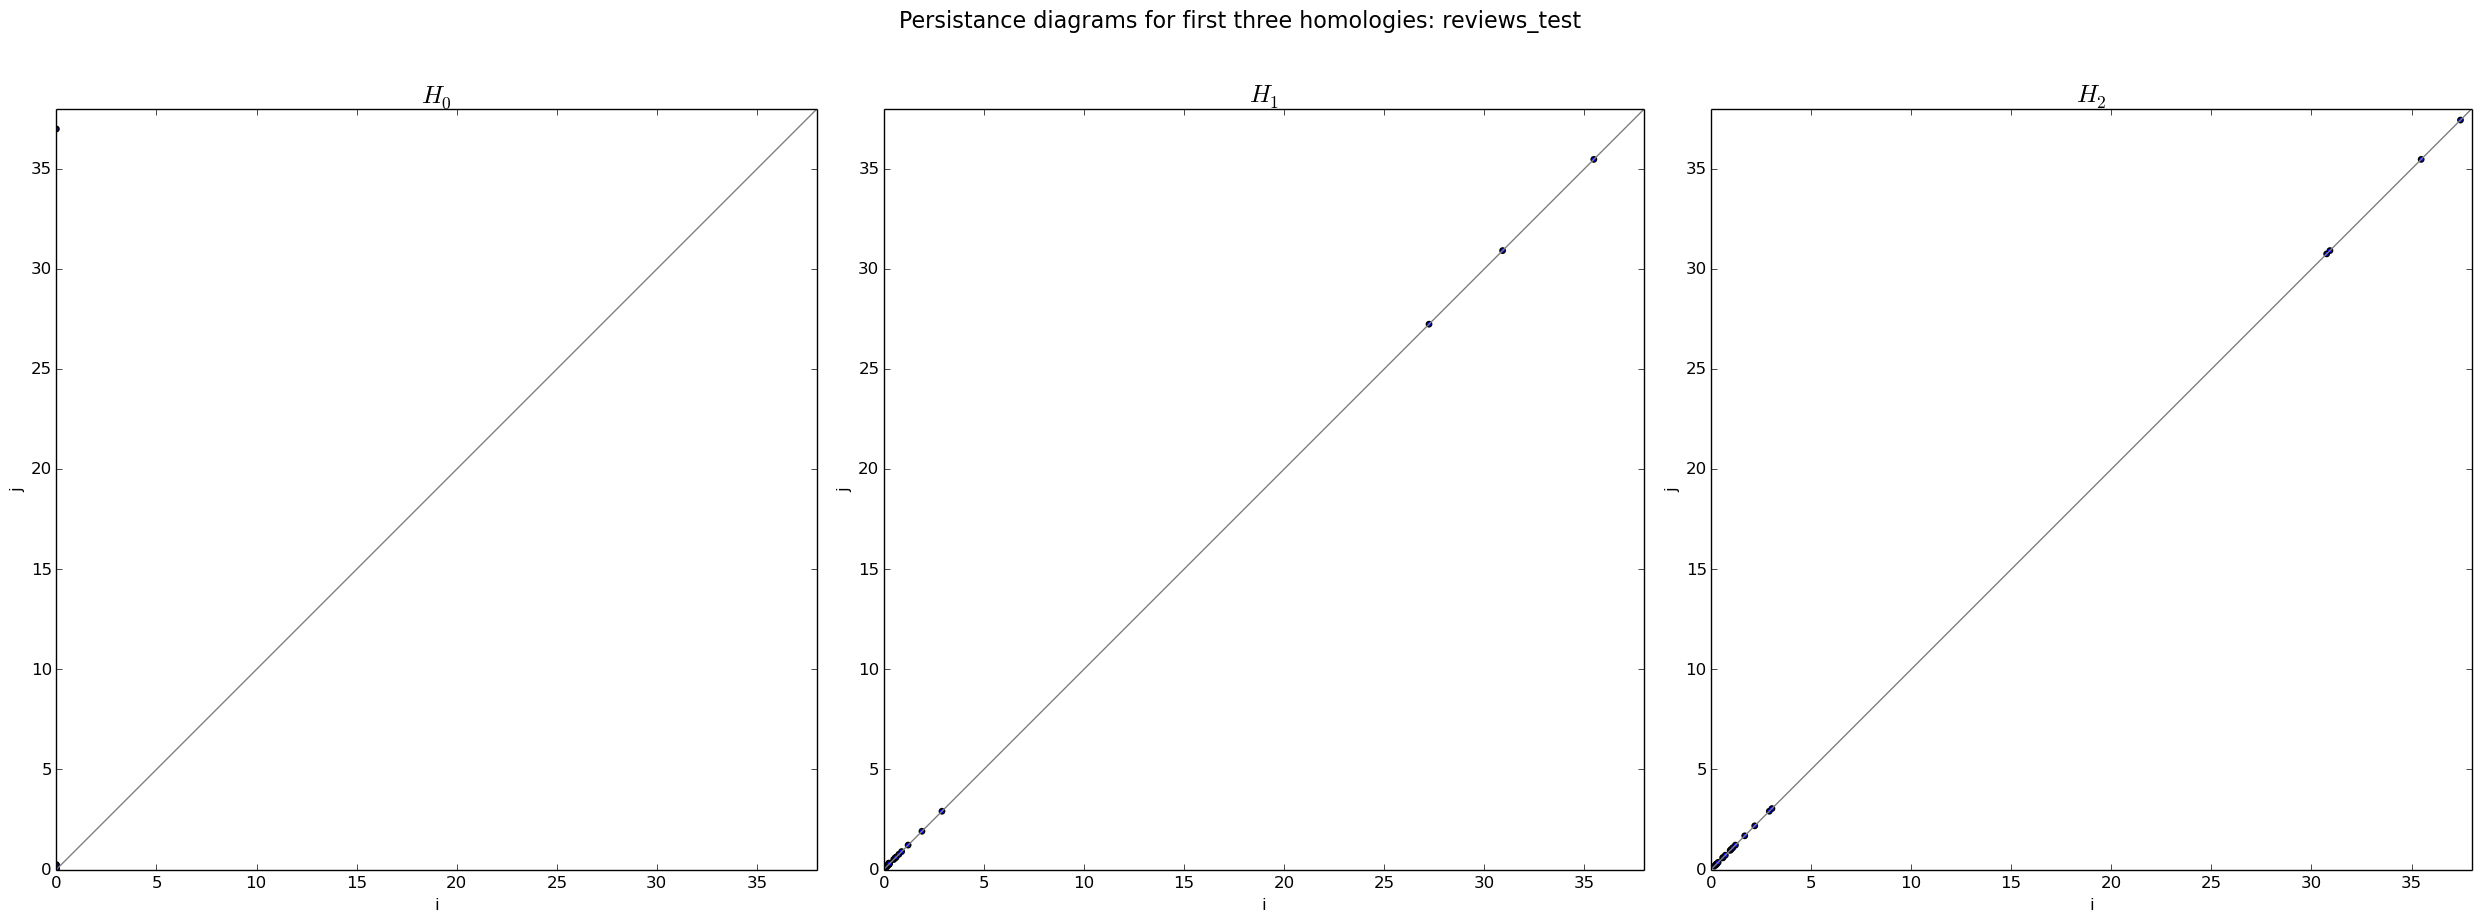
\includegraphics[width=\textwidth]{{img/pers_diagram_reviews_test.png}}
  \caption{Persistence diagrams for reviews\_test}
  \label{fig:s_4}
\end{figure}


To get concrete results on how much persistence diagrams differ between texts from different domains, we calculated bottleneck distances between all pairs of diagrams. The bottleneck distance between two diagrams is the cost of the optimal matching between points of the two diagrams. From the calculated diagrams a pairwise distance matrix was constructed, on top of which hierarchical clustering was performed. To test weather or not persistence diagrams can separate documents from different domains, we first split documents from each of the three domains into two groups. This way we obtained six groups of documents where each two of them came from the same domain. The main idea is that if persistence diagrams separate the documents from different domains well, each two groups of documents from the same domain, would be grouped ``sooner'' in the hierarchical clustering than group of documents from different domains. Results can be seen in figure~\ref{fig:h_1}. We can first notice that abstracts and sports texts get connected sooner than abstracts and sports with itself. This means that bottleneck distance between one group of sports texts and abstracts texts is smallest distance between all 6 groups. This leads to that persistence diagrams between two groups of sports articles differ more than diagrams of different domains (at least by means of bottleneck distance).


\begin{figure}[H]
  \centering
  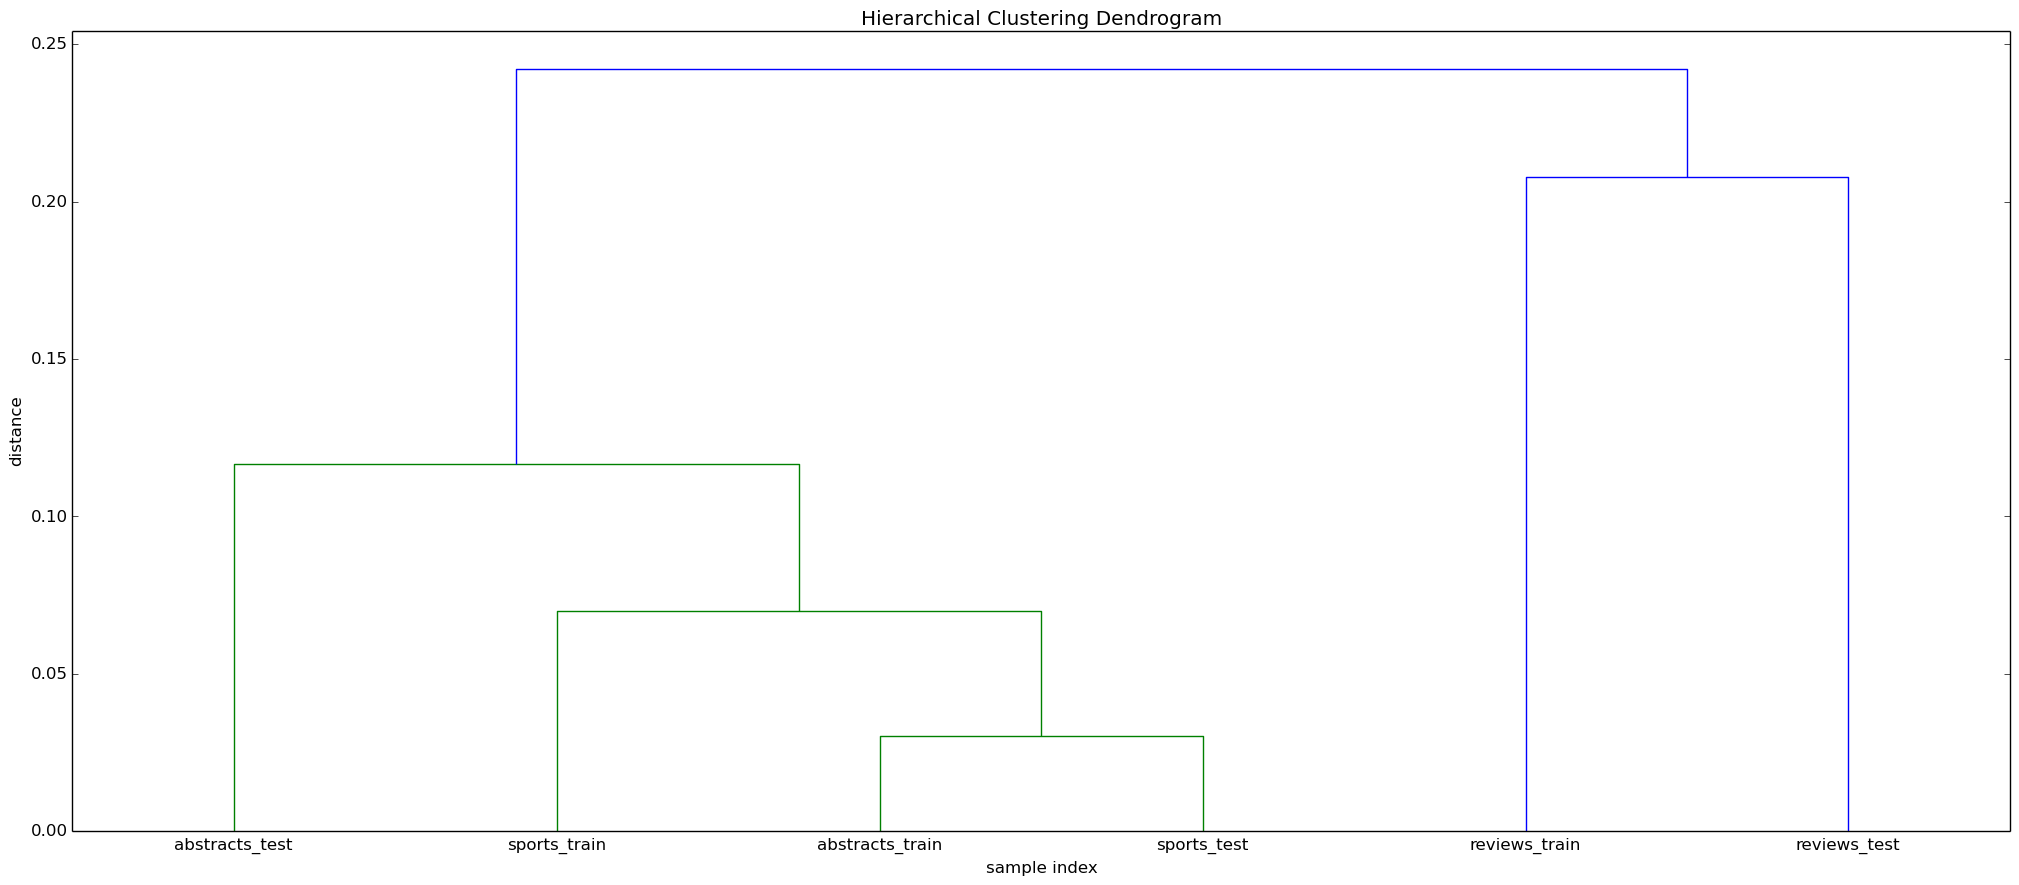
\includegraphics[width=\textwidth]{{img/histogram_main.png}}
  \caption{Hierarchical clustering results on texts dataset.}
  \label{fig:h_1}
\end{figure}

The results are not promising. One would expect that diagrams from groups of documents from same domain would differ significantly less, than diagrams of different domains, and that inner-domain bottleneck distances would therefore be much smaller. Instead of using the bottleneck distance as a distance metric between diagrams we also tested the Wasserstein distance, with no improvement in the results.


We also tested the hierarchical clustering method on a ``toy'' dataset where one sample of points were coming from a circle, and the other one form a straight line. The clustering had no trouble distinguishing between the domains and the expected results can be seen in~\ref{fig:h_2}. The inner-group bottleneck distances in both groups are much smaller than the distance between groups from different domains, which confirms the intuition of our test, and that the results would be expected of persistence diagrams differed enough.

\begin{figure}[H]
  \centering
  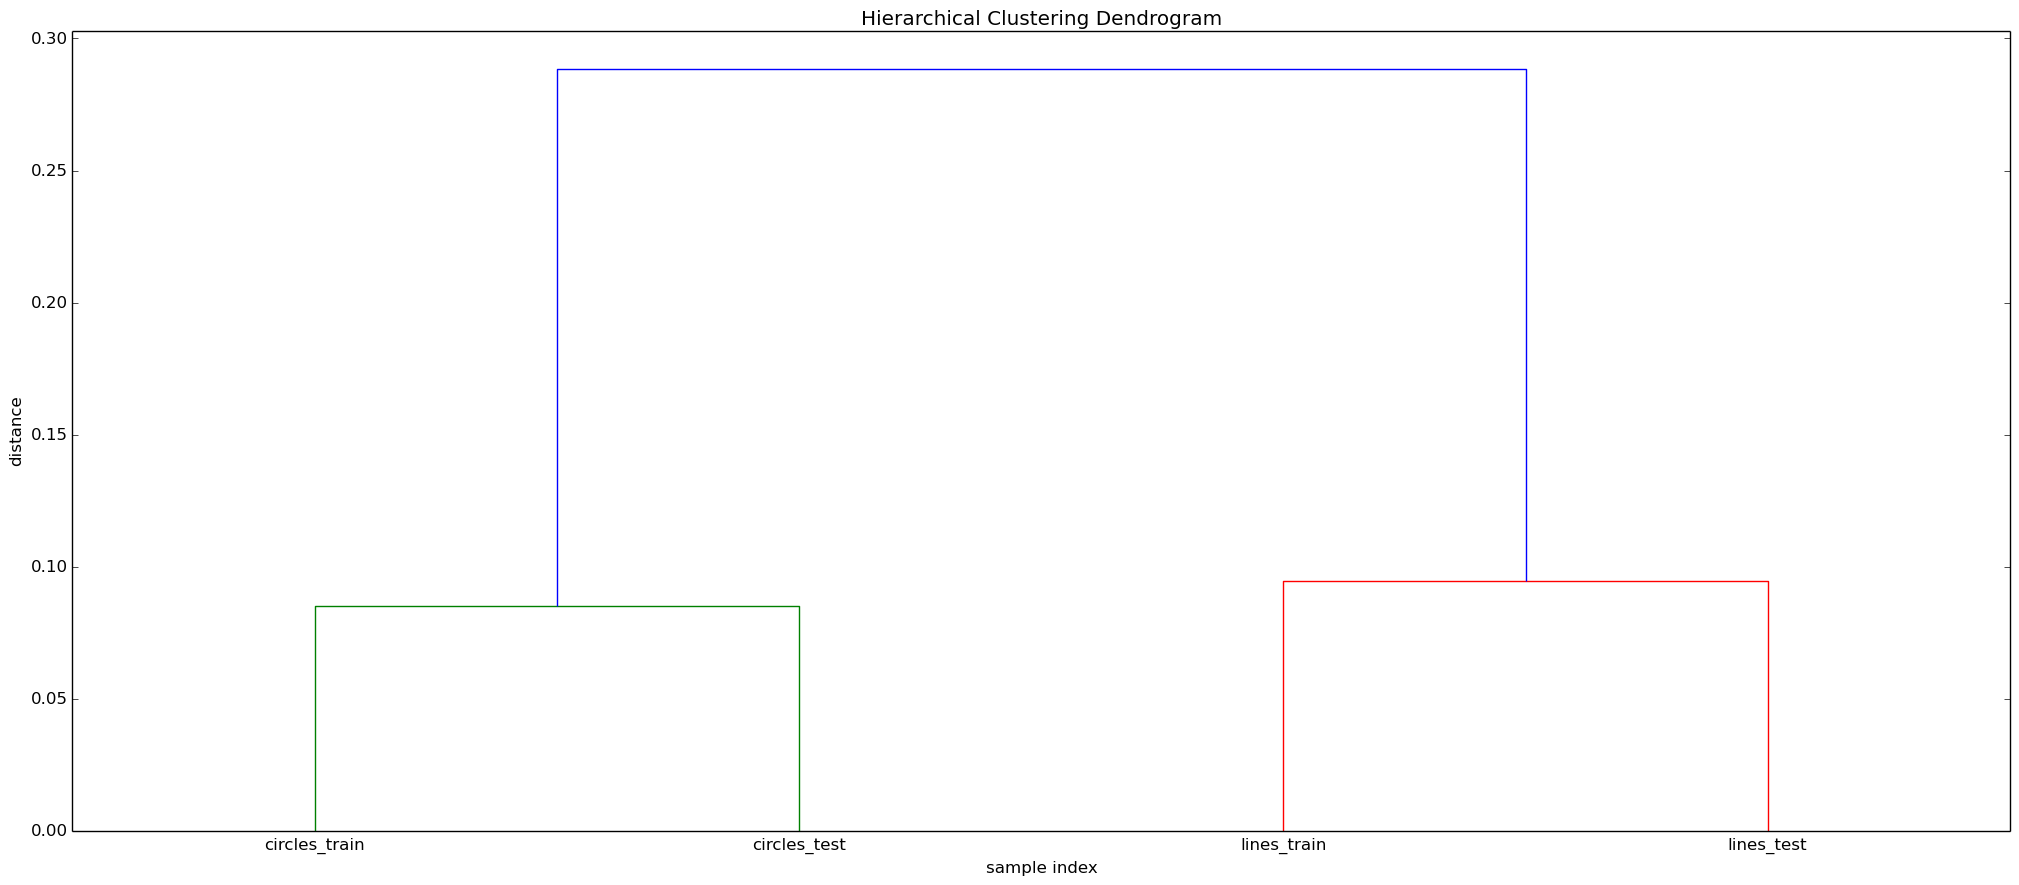
\includegraphics[width=\textwidth]{{img/histogram_toy.png}}
  \caption{Hierarchical clustering results on a toy ``circles and lines'' dataset.}
  \label{fig:h_2}
\end{figure}
